\appendix


\chapter{Detailed ADCS Simulation Models}
\label{app:adcs_detailed_models}
This appendix provides supplementary details for the ADCS simulation models used in Section~\ref{sec:adcs}. The main body of the report presents the assumptions, governing relations, parameters, and results required for the preliminary subsystem-level assessment. The present appendix collects the detailed statistical results, supplementary orbital-environment outputs, sensor-error models, actuator internal models, attitude-estimation algorithm details, and robust-control implementation details that support the main analysis.

\section{Monte Carlo Inertia Statistical Results}
\label{app:adcs_monte_carlo_inertia_statistics}

The representative inertia tensors used in the main ADCS simulations were obtained from a Monte Carlo analysis with \(10{,}000\) samples. The main body of the report summarizes the representative mass properties and inertia tensors used for the SAT-ABC and SAT-BC control simulations in Table~\ref{tab:adcs_inertia_properties}. The complete statistical results of the Monte Carlo analysis are provided in Table~\ref{tab:app_adcs_monte_carlo_inertia_statistics}.

\begin{table}[htbp]
\centering
\caption{Monte Carlo statistical analysis results for the SAT-ABC and SAT-BC inertia tensors, using \(N=10{,}000\) samples.}
\label{tab:app_adcs_monte_carlo_inertia_statistics}
\small
\begin{tabular}{lcccc}
\hline
\textbf{Parameter} & \textbf{Mean, \(\mu\)} & \textbf{Std. Dev., \(\sigma\)} & \textbf{Minimum} & \textbf{Maximum} \\ \hline
\multicolumn{5}{l}{\textit{SAT-ABC complete system}} \\ \hline
\(I_{xx}\) [kg\(\cdot\)m\(^2\)] & \(1.0307 \times 10^{-1}\) & \(6.5180 \times 10^{-3}\) & \(7.8748 \times 10^{-2}\) & \(1.2717 \times 10^{-1}\) \\
\(I_{yy}\) [kg\(\cdot\)m\(^2\)] & \(1.0324 \times 10^{-1}\) & \(6.5319 \times 10^{-3}\) & \(7.8877 \times 10^{-2}\) & \(1.2739 \times 10^{-1}\) \\
\(I_{zz}\) [kg\(\cdot\)m\(^2\)] & \(5.4242 \times 10^{-2}\) & \(3.8730 \times 10^{-3}\) & \(3.8170 \times 10^{-2}\) & \(7.0257 \times 10^{-2}\) \\
\(I_{xy}\) [kg\(\cdot\)m\(^2\)] & \(-4.5842 \times 10^{-6}\) & \(2.7254 \times 10^{-6}\) & \(-1.5333 \times 10^{-5}\) & \(9.7442 \times 10^{-6}\) \\
\(I_{xz}\) [kg\(\cdot\)m\(^2\)] & \(-2.4415 \times 10^{-4}\) & \(1.4299 \times 10^{-4}\) & \(-7.8859 \times 10^{-4}\) & \(2.7899 \times 10^{-4}\) \\
\(I_{yz}\) [kg\(\cdot\)m\(^2\)] & \(-5.0079 \times 10^{-5}\) & \(1.4272 \times 10^{-4}\) & \(-6.0003 \times 10^{-4}\) & \(5.2290 \times 10^{-4}\) \\ \hline
\multicolumn{5}{l}{\textit{SAT-BC payload subsystem}} \\ \hline
\(I_{xx}\) [kg\(\cdot\)m\(^2\)] & \(4.4358 \times 10^{-2}\) & \(3.5668 \times 10^{-3}\) & \(3.0788 \times 10^{-2}\) & \(5.8615 \times 10^{-2}\) \\
\(I_{yy}\) [kg\(\cdot\)m\(^2\)] & \(4.4356 \times 10^{-2}\) & \(3.5667 \times 10^{-3}\) & \(3.0786 \times 10^{-2}\) & \(5.8621 \times 10^{-2}\) \\
\(I_{zz}\) [kg\(\cdot\)m\(^2\)] & \(3.4150 \times 10^{-2}\) & \(3.3279 \times 10^{-3}\) & \(2.1147 \times 10^{-2}\) & \(4.8788 \times 10^{-2}\) \\
\(I_{xy}\) [kg\(\cdot\)m\(^2\)] & \(8.9099 \times 10^{-7}\) & \(1.0411 \times 10^{-6}\) & \(-3.0924 \times 10^{-6}\) & \(7.0328 \times 10^{-6}\) \\
\(I_{xz}\) [kg\(\cdot\)m\(^2\)] & \(6.7279 \times 10^{-5}\) & \(6.4721 \times 10^{-5}\) & \(-1.5532 \times 10^{-4}\) & \(3.5186 \times 10^{-4}\) \\
\(I_{yz}\) [kg\(\cdot\)m\(^2\)] & \(-1.3559 \times 10^{-4}\) & \(6.6776 \times 10^{-5}\) & \(-4.1109 \times 10^{-4}\) & \(1.1353 \times 10^{-4}\) \\ \hline
\end{tabular}
\end{table}

\section{Supplementary Orbital-Environment Results}
\label{app:adcs_supplementary_orbital_environment}

The main body of the ADCS section presents the orbital elements, reference-frame definitions, geomagnetic-field simulation, and disturbance-torque results required for the preliminary control assessment. Additional orbital-propagation outputs are included here to document the propagated satellite kinematic states and environmental acceleration components used to verify the simulation environment.

The satellite kinematic states obtained from the orbital propagation over the simulated interval are shown in Figure~\ref{fig:app_adcs_satellite_kinematics}. These profiles provide a consistency check for the propagated position and velocity histories in the GCRF frame.

\begin{figure}[htbp]
    \centering
    \begin{subfigure}[b]{0.48\linewidth}
        \centering
        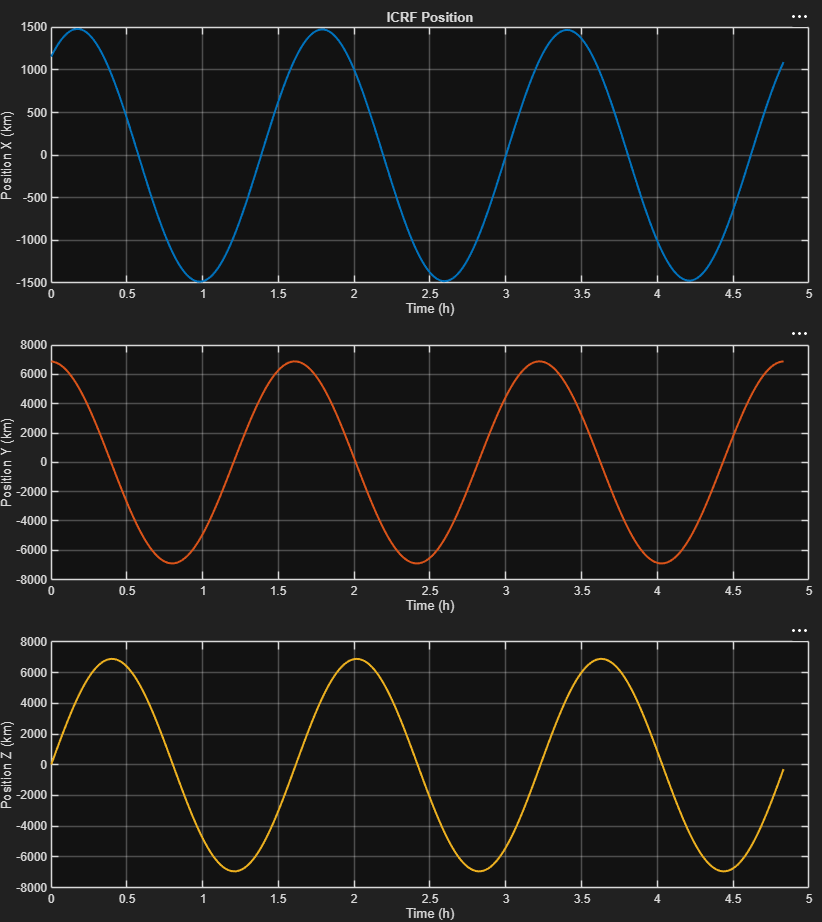
\includegraphics[width=\linewidth]{UCSP_Pictures/satellite_positions_CGRF.png}
        \caption{Satellite positions in GCRF.}
        \label{fig:app_adcs_satellite_positions}
    \end{subfigure}
    \hfill
    \begin{subfigure}[b]{0.48\linewidth}
        \centering
        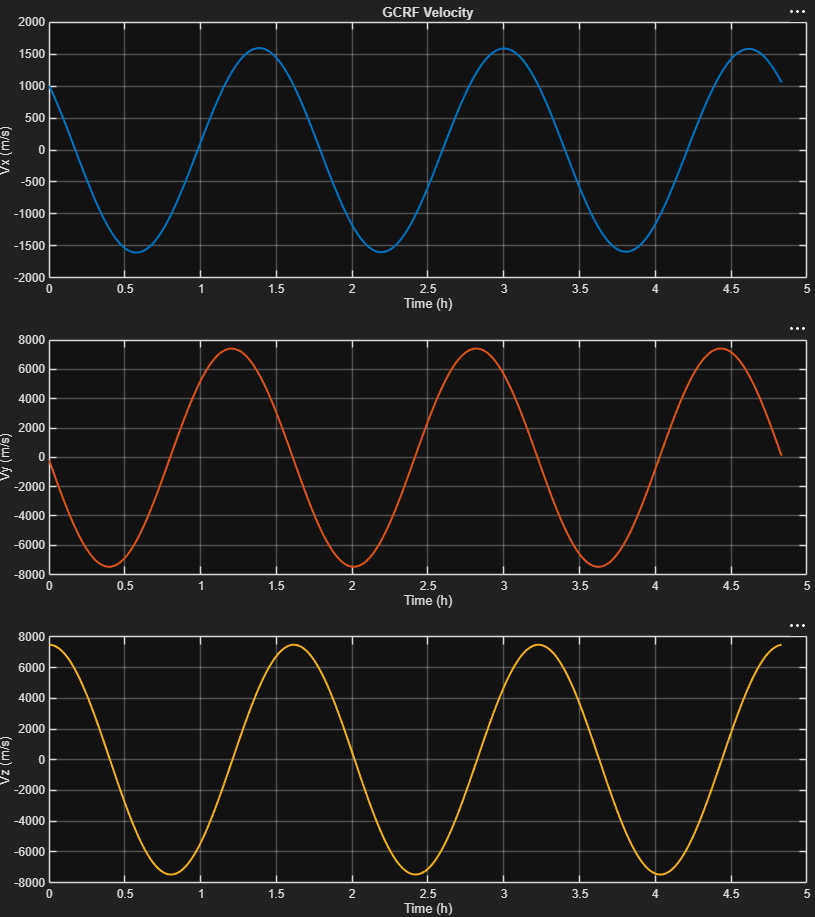
\includegraphics[width=\linewidth]{UCSP_Pictures/satellite_velocity_CGRF.png}
        \caption{Satellite velocity in GCRF.}
        \label{fig:app_adcs_satellite_velocity}
    \end{subfigure}
    \caption{Supplementary satellite kinematic states during orbital propagation.}
    \label{fig:app_adcs_satellite_kinematics}
\end{figure}

The third-body gravitational accelerations from the Moon and the Sun are shown in Figure~\ref{fig:app_adcs_third_body_perturbations}. These profiles were computed using the same Orekit-based orbital propagation model described in Section~\ref{subsub:adcs_environment}.

\begin{figure}[htbp]
    \centering
    \begin{subfigure}[b]{0.48\linewidth}
        \centering
        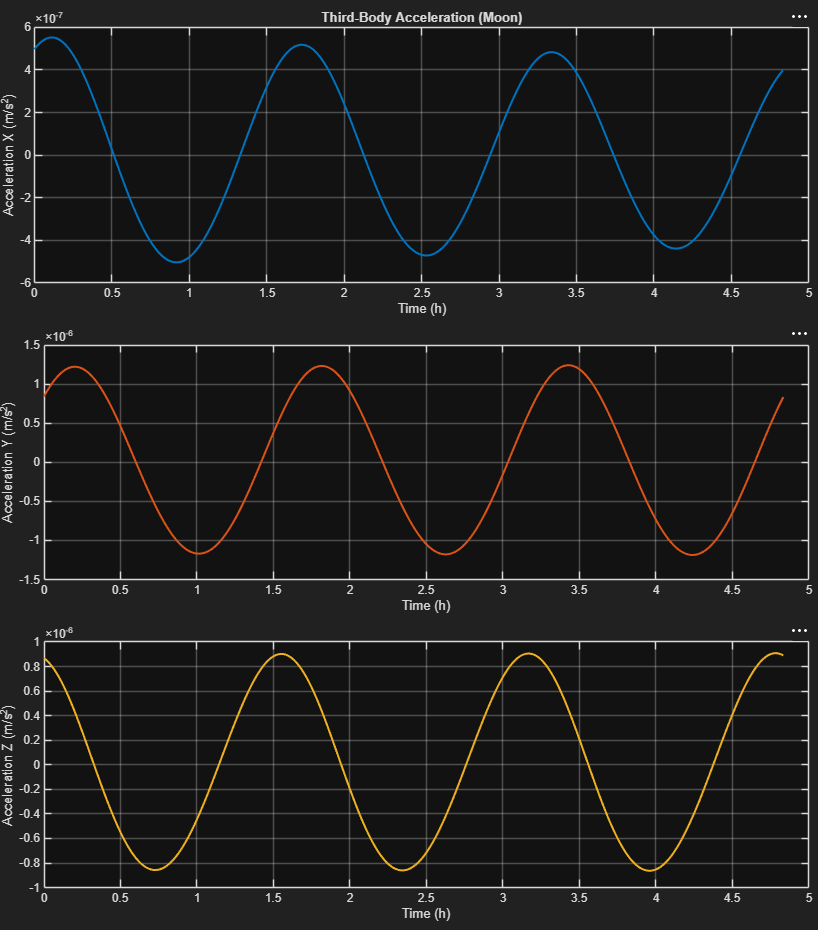
\includegraphics[width=\linewidth]{UCSP_Pictures/moonacceleration.png}
        \caption{Lunar third-body acceleration.}
        \label{fig:app_adcs_moon_acceleration}
    \end{subfigure}
    \hfill
    \begin{subfigure}[b]{0.48\linewidth}
        \centering
        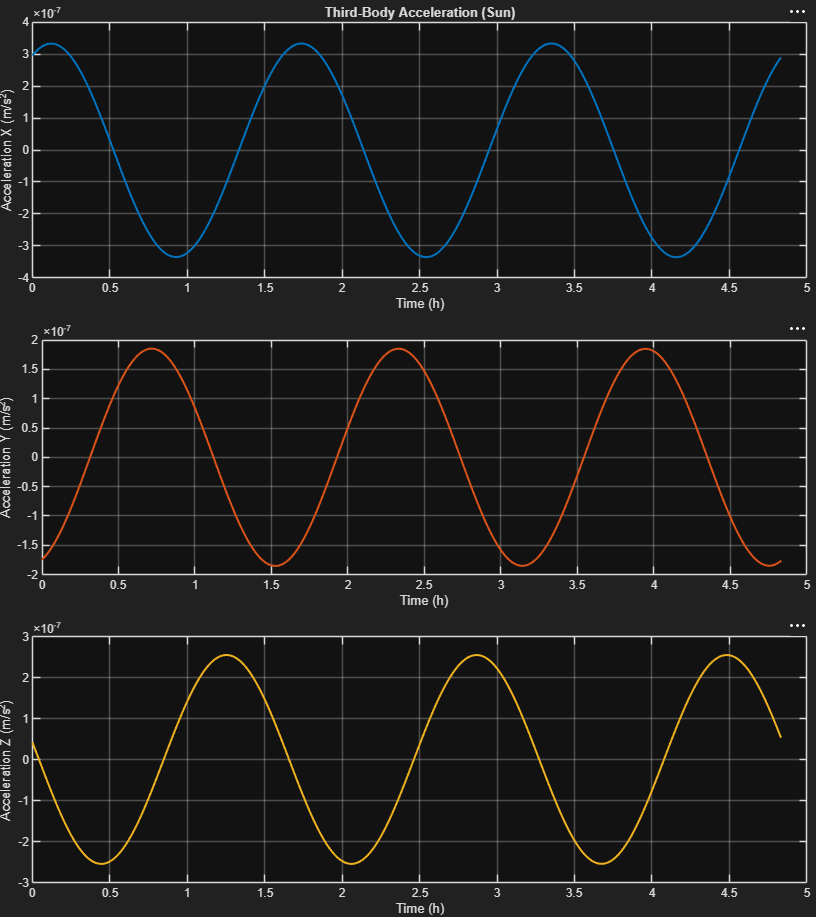
\includegraphics[width=\linewidth]{UCSP_Pictures/sunacceleration.png}
        \caption{Solar third-body acceleration.}
        \label{fig:app_adcs_sun_acceleration}
    \end{subfigure}
    \caption{Supplementary third-body gravitational perturbations acting on the satellite.}
    \label{fig:app_adcs_third_body_perturbations}
\end{figure}

The non-gravitational acceleration components associated with solar radiation pressure and atmospheric drag are shown in Figure~\ref{fig:app_adcs_non_gravitational_perturbations}. These acceleration histories support the environmental disturbance-torque assessment summarized in the main ADCS section.

\begin{figure}[htbp]
    \centering
    \begin{subfigure}[b]{0.48\linewidth}
        \centering
        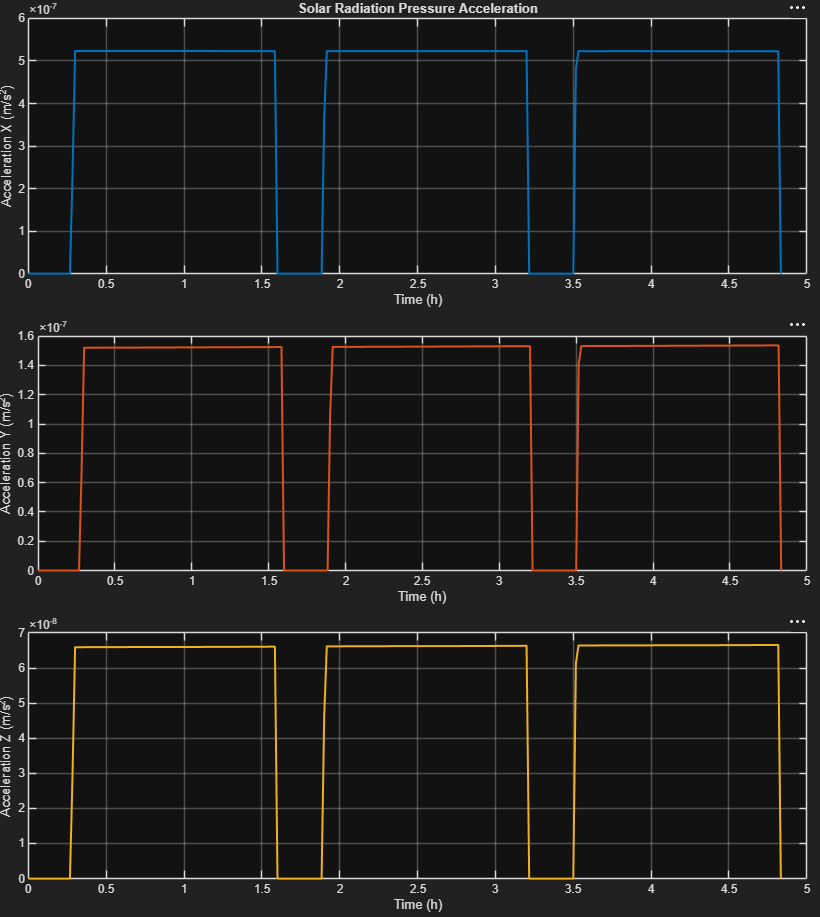
\includegraphics[width=\linewidth]{UCSP_Pictures/solar_rad-acceleration.png}
        \caption{Solar radiation pressure acceleration.}
        \label{fig:app_adcs_solar_radiation_acc}
    \end{subfigure}
    \hfill
    \begin{subfigure}[b]{0.48\linewidth}
        \centering
        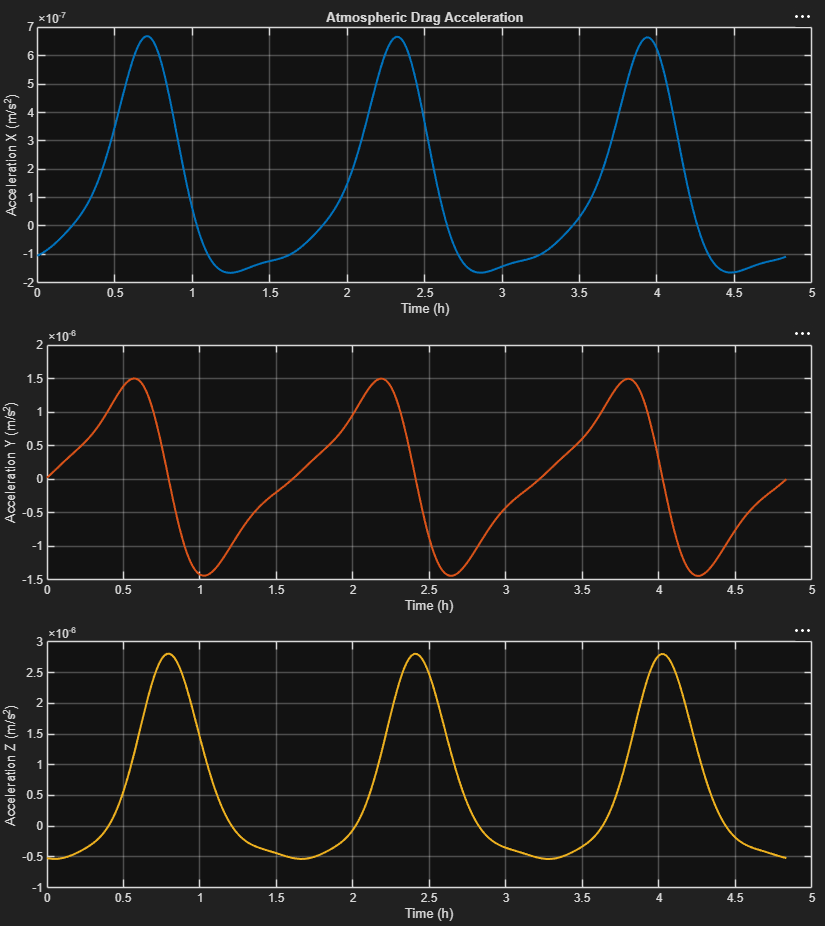
\includegraphics[width=\linewidth]{UCSP_Pictures/satellite_drag_acceleration_CGRF.png}
        \caption{Atmospheric drag acceleration in GCRF.}
        \label{fig:app_adcs_atmospheric_drag_acc}
    \end{subfigure}
    \caption{Supplementary non-gravitational acceleration perturbations acting on the satellite.}
    \label{fig:app_adcs_non_gravitational_perturbations}
\end{figure}

Because the SAT-ABC and SAT-BC configurations remain in close orbital proximity during the active pre-separation stages, the same orbital propagation model and environmental acceleration profiles are used for both configurations in the preliminary ADCS simulations.

\section{Detailed Sensor Models}
\label{app:adcs_detailed_sensor_models}

The main ADCS section summarizes the governing sensor relations used in the attitude-determination and control simulations. The detailed sensor-error model is described here for traceability.

\subsection{IMU Error Model}
\label{app:adcs_imu_error_model}

The IMU model includes scale-factor errors, axis misalignment, bias instability, additive measurement noise, filtering, saturation, and ADC quantization. The scale-factor and axis-misalignment matrices are defined as

\begin{equation}
    \mathbf{T}_{\mathrm{sf}}
    =
    \begin{bmatrix}
        1+s_x & 0 & 0 \\
        0 & 1+s_y & 0 \\
        0 & 0 & 1+s_z
    \end{bmatrix},
    \qquad
    \mathbf{T}_{\mathrm{ma}}
    =
    \begin{bmatrix}
        1 & m_{yx} & m_{zx} \\
        m_{xy} & 1 & m_{zy} \\
        m_{xz} & m_{yz} & 1
    \end{bmatrix},
    \label{eq:app_adcs_scale_misalignment_matrices}
\end{equation}

where \(s_x\), \(s_y\), and \(s_z\) are scale-factor errors for each axis, and \(m_{ij}\) represents the angular deviation of axis \(i\) with respect to axis \(j\). The raw gyroscope measurement is modeled as

\begin{equation}
    \tilde{\boldsymbol{\omega}}_{\mathrm{raw}}(t)
    =
    \mathbf{T}_{\mathrm{ma}}
    \mathbf{T}_{\mathrm{sf}}
    \boldsymbol{\omega}(t)
    +
    \mathbf{b}_{g}(t)
    +
    \boldsymbol{\eta}_{g}(t),
    \label{eq:app_adcs_gyro_raw_measurement}
\end{equation}

where \(\boldsymbol{\omega}(t)\) is the true angular velocity, \(\mathbf{b}_{g}(t)\) is the gyroscope bias, and \(\boldsymbol{\eta}_{g}(t)\) is additive gyroscope noise. The bias is propagated using the random-walk model

\begin{equation}
    \mathbf{b}_{g}(t)
    =
    \mathbf{b}_{g}(t-\Delta t)
    +
    \boldsymbol{\eta}_{bg},
    \label{eq:app_adcs_gyro_bias_random_walk}
\end{equation}

where \(\boldsymbol{\eta}_{bg}\) is a Gaussian noise process with standard deviation \(\sigma_{\mathrm{RW}}\sqrt{\Delta t}\). A first-order low-pass filter is applied to the raw gyroscope output as

\begin{equation}
    \tilde{\boldsymbol{\omega}}_{\mathrm{filt}}(k)
    =
    (1-\alpha)
    \tilde{\boldsymbol{\omega}}_{\mathrm{filt}}(k-1)
    +
    \alpha
    \tilde{\boldsymbol{\omega}}_{\mathrm{raw}}(k),
    \label{eq:app_adcs_gyro_low_pass_filter}
\end{equation}

with

\begin{equation}
    \alpha
    =
    \frac{T_s}{\tau + T_s},
    \label{eq:app_adcs_filter_alpha}
\end{equation}

where \(T_s\) is the sampling time and \(\tau\) is the filter time constant.

\subsection{Vector Measurement Models}
\label{app:adcs_vector_measurement_models}

The accelerometer and magnetometer measurements are modeled by rotating the corresponding inertial-frame reference vectors into the body frame and applying the same scale-factor and misalignment structure used for the IMU model. The accelerometer measurement is given by

\begin{equation}
    \tilde{\mathbf{f}}_{\mathrm{raw}}
    =
    \mathbf{T}_{\mathrm{ma}}
    \mathbf{T}_{\mathrm{sf}}
    \left(
        \mathbf{R}(\mathbf{q})^{T}
        \mathbf{g}_{I}
    \right)
    +
    \mathbf{b}_{a}
    +
    \boldsymbol{\eta}_{a},
    \label{eq:app_adcs_accelerometer_model}
\end{equation}

where \(\mathbf{g}_{I}\) is the inertial-frame reference vector, \(\mathbf{b}_{a}\) is the accelerometer bias, and \(\boldsymbol{\eta}_{a}\) is accelerometer measurement noise. The magnetometer measurement is modeled as

\begin{equation}
    \tilde{\mathbf{m}}_{\mathrm{raw}}
    =
    \mathbf{T}_{\mathrm{ma}}
    \mathbf{T}_{\mathrm{sf}}
    \left(
        \mathbf{R}(\mathbf{q})^{T}
        \mathbf{m}_{I}
    \right)
    +
    \mathbf{b}_{m}
    +
    \boldsymbol{\eta}_{m},
    \label{eq:app_adcs_magnetometer_model}
\end{equation}

where \(\mathbf{m}_{I}\) is the inertial-frame geomagnetic-field reference vector, \(\mathbf{b}_{m}\) is the magnetometer bias, and \(\boldsymbol{\eta}_{m}\) is magnetometer noise.

The Sun sensor is represented as a reference-vector measurement. Its measured vector is modeled as

\begin{equation}
    \tilde{\mathbf{s}}_{\mathrm{meas}}
    =
    \mathbf{R}(\mathbf{q})^{T}
    \mathbf{s}_{I}
    +
    \mathbf{b}_{\mathrm{sun}}
    +
    \boldsymbol{\eta}_{\mathrm{sun}},
    \label{eq:app_adcs_sun_sensor_model}
\end{equation}

where \(\mathbf{s}_{I}\) is the true line-of-sight vector to the Sun expressed in the inertial frame, \(\mathbf{b}_{\mathrm{sun}}\) is the Sun-sensor bias, and \(\boldsymbol{\eta}_{\mathrm{sun}}\) is the corresponding Gaussian noise term.

\subsection{Saturation and ADC Quantization}
\label{app:adcs_sensor_adc_quantization}

To account for physical hardware limitations, sensor outputs are passed through saturation and quantization stages. The raw physical signal vector \(\mathbf{y}\in\mathbb{R}^{3}\) is first bounded element-wise by the sensor operational limits, \(y_{\min}\) and \(y_{\max}\), producing the saturated vector \(\mathbf{y}_{\mathrm{sat}}\). This vector is mapped to an analog input voltage as

\begin{equation}
    \mathbf{V}_{\mathrm{in}}
    =
    \frac{
        V_{\mathrm{ref}}
    }{
        y_{\max} - y_{\min}
    }
    \left(
        \mathbf{y}_{\mathrm{sat}}
        -
        y_{\min}
        \mathbf{1}_{3\times1}
    \right),
    \label{eq:app_adcs_sensor_saturation_voltage}
\end{equation}

where \(V_{\mathrm{ref}}\) is the ADC reference voltage and \(\mathbf{1}_{3\times1}=[1,1,1]^T\). The analog voltage is then quantized into an integer digital vector according to

\begin{equation}
    \mathbf{D}_{\mathrm{out}}
    =
    \operatorname{round}
    \left(
        \frac{
            2^{n_{\mathrm{bits}}}-1
        }{
            V_{\mathrm{ref}}
        }
        \mathbf{V}_{\mathrm{in}}
    \right),
    \label{eq:app_adcs_adc_digital_output}
\end{equation}

where \(n_{\mathrm{bits}}\) is the ADC resolution. The physical value reintroduced into the simulation is reconstructed as

\begin{equation}
    \mathbf{y}_{\mathrm{out}}
    =
    y_{\min}
    \mathbf{1}_{3\times1}
    +
    \frac{
        y_{\max} - y_{\min}
    }{
        2^{n_{\mathrm{bits}}}-1
    }
    \mathbf{D}_{\mathrm{out}}.
    \label{eq:app_adcs_adc_reconstructed_output}
\end{equation}

\section{Detailed Actuator Models}
\label{app:adcs_detailed_actuator_models}

\subsection{Reaction-Wheel Assembly Model}
\label{app:adcs_reaction_wheel_model}

The reaction-wheel assembly is modeled as an array of \(N\) reaction wheels. Each wheel includes a closed-loop PID speed controller coupled to the electrical and mechanical dynamics of a DC motor. For the \(j\)-th wheel, the mechanical and electrical dynamics are represented by

\begin{align}
    \dot{\omega}_{\mathrm{rw},j}
    &=
    \frac{1}{J_{\mathrm{rw}}}
    \left(
        k_t i_j
        -
        B\omega_{\mathrm{rw},j}
        -
        K_c
        \operatorname{sign}(\omega_{\mathrm{rw},j})
    \right),
    \label{eq:app_adcs_rw_mechanical} \\
    \dot{i}_{j}
    &=
    \frac{1}{L}
    \left(
        u_j
        -
        R i_j
        -
        K_e\omega_{\mathrm{rw},j}
    \right),
    \label{eq:app_adcs_rw_electrical}
\end{align}

where \(\omega_{\mathrm{rw},j}\) and \(i_j\) are the angular rate and current of the \(j\)-th reaction wheel. The shared motor parameters are:

\begin{itemize}
    \item \(L\) and \(R\): armature inductance and resistance;
    \item \(K_e\) and \(k_t\): back-EMF and motor torque constants;
    \item \(J_{\mathrm{rw}}\): rotor inertia;
    \item \(B\) and \(K_c\): viscous and Coulomb friction coefficients.
\end{itemize}

The internal PID controller tracks the reference speed and computes an unbounded voltage command, \(u_{\mathrm{unb}}\). This command is saturated to the applied voltage \(u_{\mathrm{app}}\in[-V_{\max},V_{\max}]\) using a clamping anti-windup mechanism. The motor dynamics are solved using a fourth-order Runge--Kutta method, and the state vector \(\mathbf{x}=[\omega_{\mathrm{rw},j}, i_j]^T\) is constrained by the wheel-speed and current limits, \(\omega_{\mathrm{rw,max}}\) and \(i_{\mathrm{rw,max}}\).

The true mechanical torque generated by the \(j\)-th wheel is derived from the wheel momentum rate of change:

\begin{equation}
    \tau_{\mathrm{real},j}
    =
    J_{\mathrm{rw}}
    \frac{
        \omega_{\mathrm{rw},j}(t)
        -
        \omega_{\mathrm{rw},j}(t-\Delta t)
    }{
        \Delta t
    }.
    \label{eq:app_adcs_rw_real_torque}
\end{equation}

The individual wheel torques are projected onto the satellite body frame using the reaction-wheel configuration matrix \(\mathbf{W}_{\mathrm{rw}}\).

\subsection{Magnetorquer Assembly Model}
\label{app:adcs_magnetorquer_model}

The magnetorquer assembly maps commanded magnetic dipoles into body-frame magnetic control torques while accounting for magnetic and electrical constraints. The commanded dipole vector, \(\mathbf{m}_{\mathrm{cmd}}\), is first limited by the physical saturation of the magnetic core, producing a saturated dipole vector \(\mathbf{m}_{\mathrm{sat}}\). The required coil voltage is estimated from Ohm's law as

\begin{equation}
    \mathbf{V}_{\mathrm{req}}
    =
    \frac{
        \mathbf{m}_{\mathrm{sat}}
    }{
        K_m
    }
    R_m,
    \label{eq:app_adcs_mtq_required_voltage}
\end{equation}

where \(R_m\) is the internal resistance of the coil and \(K_m\) is the current-to-dipole conversion factor. The required voltage is limited by the maximum bus voltage to obtain the applied voltage \(\mathbf{V}_{\mathrm{app}}\). The realized magnetic dipole is then

\begin{equation}
    \mathbf{m}_{\mathrm{real}}
    =
    K_m
    \left(
        \frac{
            \mathbf{V}_{\mathrm{app}}
        }{
            R_m
        }
    \right).
    \label{eq:app_adcs_mtq_real_dipole}
\end{equation}

The individual coil dipoles are mapped to the satellite body frame using the magnetorquer configuration matrix \(\mathbf{W}_{\mathrm{mtq}}\). The resulting magnetic control torque is

\begin{equation}
    \boldsymbol{\tau}_{\mathrm{mtq}}
    =
    \left(
        \mathbf{W}_{\mathrm{mtq}}
        \mathbf{m}_{\mathrm{real}}
    \right)
    \times
    \mathbf{B}_{\mathrm{body}},
    \label{eq:app_adcs_mtq_control_torque}
\end{equation}

where \(\mathbf{B}_{\mathrm{body}}\) is the local geomagnetic-field vector expressed in the satellite body frame.

\section{Detailed Attitude-Estimation Algorithm Descriptions}
\label{app:adcs_attitude_estimation_algorithms}

This section provides additional mathematical and implementation details for the attitude-estimation algorithms summarized in Section~\ref{subsub:adcs_satabc_attitude_determination}. These algorithms were considered as candidate AHRS approaches during the SAT-ABC settling interval.

\subsection{QUEST}
\label{app:adcs_quest_algorithm}

QUEST is a deterministic vector-based solution to Wahba's problem. It constructs Davenport's \(K\)-matrix from weighted body-frame vector observations and their corresponding inertial-frame reference vectors. The implementation computes the gain matrix \(B\) and the error vector \(z\), which are used to assemble a symmetric \(4\times4\) matrix. The eigenvector associated with the largest eigenvalue provides the optimal attitude quaternion. Since QUEST is a measurement-only method, it provides an attitude estimate independently of gyroscope propagation.

\subsection{RE-QUEST}
\label{app:adcs_request_algorithm}

RE-QUEST extends QUEST by recursively propagating attitude information using gyroscope measurements and updating it with vector observations. The algorithm maintains an accumulated matrix \(K_{\mathrm{acc}}\) and a total accumulated weight \(m_{\mathrm{acc}}\). A fading-memory factor \(P\) is used to prioritize recent data. During the predict step, the accumulated matrix is propagated using a transition matrix \(\boldsymbol{\Phi}\) derived from angular-rate measurements. During the update step, the current batch of vector measurements is blended into the accumulated information matrix. The attitude quaternion is then extracted as the principal eigenvector of the updated \(K\)-matrix.

\subsection{Mahony Filter}
\label{app:adcs_mahony_filter}

The Mahony filter is a nonlinear complementary filter that fuses gyroscope measurements with vector observations through proportional-integral feedback. The filter computes an attitude-error vector by comparing measured body-frame vectors with predicted directions derived from the current attitude estimate and the inertial-frame reference vectors. The proportional gain \(K_P\) provides instantaneous attitude correction, while the integral gain \(K_I\) supports gyroscope-bias estimation and compensation. The method operates directly on the quaternion attitude representation and is suitable for embedded applications due to its relatively low computational cost.

\subsection{Madgwick Filter}
\label{app:adcs_madgwick_filter}

The Madgwick filter estimates the attitude quaternion, \(\mathbf{q}_{\mathrm{est},t}\), and gyroscope bias, \(\mathbf{b}_{g,\mathrm{est}}\), by combining gyroscope-based propagation with a gradient-descent correction based on vector observations. The prediction step integrates the measured angular velocity, \(\tilde{\boldsymbol{\omega}}_{\mathrm{meas}}\), to obtain a propagated quaternion estimate, \(\mathbf{q}_{\omega,t}\). The correction step minimizes the mismatch between measured vectors, such as \(\tilde{\mathbf{f}}_{\mathrm{meas}}\), \(\tilde{\mathbf{m}}_{\mathrm{meas}}\), and optionally \(\tilde{\mathbf{s}}_{\mathrm{meas},n}\), and their corresponding predicted reference directions.

The correction direction is computed from the normalized gradient of an objective function. The final estimated quaternion rate is obtained by combining the gyroscope propagation and gradient-descent correction:

\begin{equation}
    \dot{\mathbf{q}}_{\mathrm{est},t}
    =
    \dot{\mathbf{q}}_{\omega,t}
    -
    \beta
    \dot{\mathbf{q}}_{\epsilon,t},
    \label{eq:app_adcs_madgwick_estimated_rate}
\end{equation}

where \(\dot{\mathbf{q}}_{\omega,t}\) is the quaternion rate obtained from gyroscope propagation, \(\dot{\mathbf{q}}_{\epsilon,t}\) is the normalized correction direction, and \(\beta\) is the filter gain. The implementation considered for LINKU separates the logic into predict and update methods, which supports high-frequency attitude propagation and allows additional reference vectors, such as star-tracker measurements, to be incorporated in the objective function.

\subsection{Extended Kalman Filter}
\label{app:adcs_ekf_filter}

The EKF is implemented as a full-state nonlinear estimator with state vector

\begin{equation}
    \mathbf{x}
    =
    \begin{bmatrix}
        \mathbf{q}^{T} &
        \mathbf{b}_{g}^{T}
    \end{bmatrix}^{T},
    \label{eq:app_adcs_ekf_state}
\end{equation}

where \(\mathbf{q}\) is the attitude quaternion and \(\mathbf{b}_{g}\) is the gyroscope bias. The state uncertainty is represented by the covariance matrix \(\mathbf{P}\in\mathbb{R}^{7\times7}\). The measurement model uses inertial reference vectors transformed into the body frame:

\begin{equation}
    \mathbf{y}
    =
    \mathbf{R}(\mathbf{q})^{T}
    \mathbf{v}_{\mathrm{ref}},
    \label{eq:app_adcs_ekf_measurement_model}
\end{equation}

where \(\mathbf{v}_{\mathrm{ref}}\) is a reference vector expressed in the inertial frame. The predict step propagates the attitude estimate using gyroscope measurements, while the correction step updates the state when new sensor measurements are available. The additive update has the form

\begin{equation}
    \mathbf{x}_{t}
    =
    \mathbf{x}_{t-\Delta t}
    +
    \mathbf{K}
    \left(
        \mathbf{y}_{\mathrm{meas}}
        -
        \mathbf{y}_{\mathrm{est}}
    \right),
    \label{eq:app_adcs_ekf_additive_update}
\end{equation}

where \(\mathbf{K}\) is the Kalman gain. After the additive update, the quaternion component of the state is re-normalized.

\subsection{Unscented Kalman Filter}
\label{app:adcs_ukf_filter}

The UKF estimates the attitude quaternion while representing uncertainty through a three-dimensional rotation-error covariance matrix, \(\mathbf{P}\in\mathbb{R}^{3\times3}\). The attitude error is represented by an axis-angle rotation vector,

\begin{equation}
    \boldsymbol{\delta\theta}
    =
    \vartheta \mathbf{e},
    \label{eq:app_adcs_ukf_rotation_error}
\end{equation}

where \(\vartheta\) is the error angle and \(\mathbf{e}\) is the corresponding unit rotation axis. The predict step propagates a set of sigma points, \(\chi_i\), through the quaternion kinematic model using the measured angular velocity, \(\tilde{\boldsymbol{\omega}}_{\mathrm{meas}}\). During the correction step, the propagated sigma points are transformed into the measurement space using

\begin{equation}
    \mathbf{y}
    =
    \mathbf{R}(\mathbf{q})^{T}
    \mathbf{v}_{\mathrm{ref}}.
    \label{eq:app_adcs_ukf_measurement_model}
\end{equation}

The predicted measurements are compared with the actual measurements, such as \(\tilde{\mathbf{f}}_{\mathrm{meas}}\), \(\tilde{\mathbf{m}}_{\mathrm{meas}}\), and optionally \(\tilde{\mathbf{s}}_{\mathrm{meas},n}\). The resulting innovation is used to compute the Kalman gain and apply a multiplicative correction to the attitude state.

\section{Boskovic Robust Controller Adaptive-Gain Law}
\label{app:adcs_boskovic_adaptive_gain}

The main body of the ADCS section presents the Boskovic robust controller through the control law and sliding vector used in the SAT-ABC velocity-vector pointing assessment. The full adjustment law for the time-varying adaptive gain is provided here for completeness.

The sliding vector is defined as

\begin{equation}
    \mathbf{s}(t)
    =
    \delta\boldsymbol{\omega}(t)
    +
    k^2(t)
    \delta\mathbf{q}_{13}(t),
    \label{eq:app_adcs_boskovic_sliding_vector}
\end{equation}

where \(\delta\boldsymbol{\omega}(t)\) is the angular-rate tracking error and \(\delta\mathbf{q}_{13}(t)\) is the vector part of the quaternion attitude error. The adaptive-gain adjustment law is

\begin{multline}
    \dot{k}(t)
    =
    \frac{
        \gamma k(t)
    }{
        1
        +
        4\gamma
        \left[
            1-\delta q_{4}(t)
        \right]
    }
    \left\{
    u_{\max}
    \sum_{i=1}^{3}
    \left[
        \frac{
            \delta\omega_i(t)\delta q_i(t)
        }{
            |s_i(t)| + k^2(t)\delta_k
        }
        -
        \frac{
            |\delta\omega_i(t)|(1+\delta_k)
        }{
            |\delta\omega_i(t)| + k^2(t)(1+\delta_k)
        }
    \right]
    \right. \\
    \left.
    -
    \delta\boldsymbol{\omega}^{T}
    \delta\mathbf{q}_{13}
    -
    k^2(t)
    \delta\mathbf{q}_{13}^{T}
    \delta\mathbf{q}_{13}
    \right\},
    \label{eq:app_adcs_boskovic_adaptive_gain}
\end{multline}

where \(\gamma\) is a positive scalar convergence-rate parameter, \(\delta_k\) is a positive constant, \(u_{\max}\) is the control-torque limit, \(\delta q_4(t)\) is the scalar part of the quaternion attitude error, and \(s_i(t)\), \(\delta\omega_i(t)\), and \(\delta q_i(t)\) are the \(i\)-th components of the sliding vector, angular-rate tracking error, and quaternion vector error, respectively.






\begin{comment}
\chapter{Separation Systems State of the Art}
\label{app:separation_systems}

A state-of-the-art review of separation systems used in aerospace applications was conducted to identify functional technological solutions, design criteria, and mechanical configurations employed in similar missions. The review considered spring-based systems, thermal release mechanisms, pyrotechnic devices, magnetic retention concepts, and electromechanical actuators. The main purpose was to extract design references applicable to the SAT-B/SAT-C separation mechanism, with emphasis on reliability, simplicity, compactness, and compatibility with the LINKU mission constraints.

\section{Motorized Lightband MkII}
\label{appsec:motorized_lightband_mkii}

The Motorized Lightband MkII (MLB MkII) is a motorized, non-pyrotechnic, space-grade separation system designed to mate and release payloads with high precision and low mass \cite{RocketLab2024MLB}. Its operation is based on an electromechanical assembly powered through a DE-9 connector, with a typical operating voltage between \(24\) and \(32~\mathrm{V}\).

The separation mechanism uses preload springs that provide the required force for payload ejection. These springs are restrained by a retention ring that keeps both halves of the system together through a series of flexible tabs distributed along the ring. The release of the ring is controlled by a linear actuator driven by two DC motors, which transmit motion through a bevel gear and ball screw system. When the separation signal is received, the actuator moves a linear guide toward the center of the separation ring, reducing its diameter. This motion releases the tabs that secure the payload, allowing the springs to propel the satellite away from the launch vehicle stage.

The MLB MkII has been widely used in space missions and, according to its manual, has successfully performed hundreds of separations aboard several launch vehicles, including Delta II, Atlas V, Falcon, Electron, Vega, Soyuz, the Space Shuttle, and PSLV, with no reported on-orbit separation failures.

\begin{figure}[htbp]
    \centering
    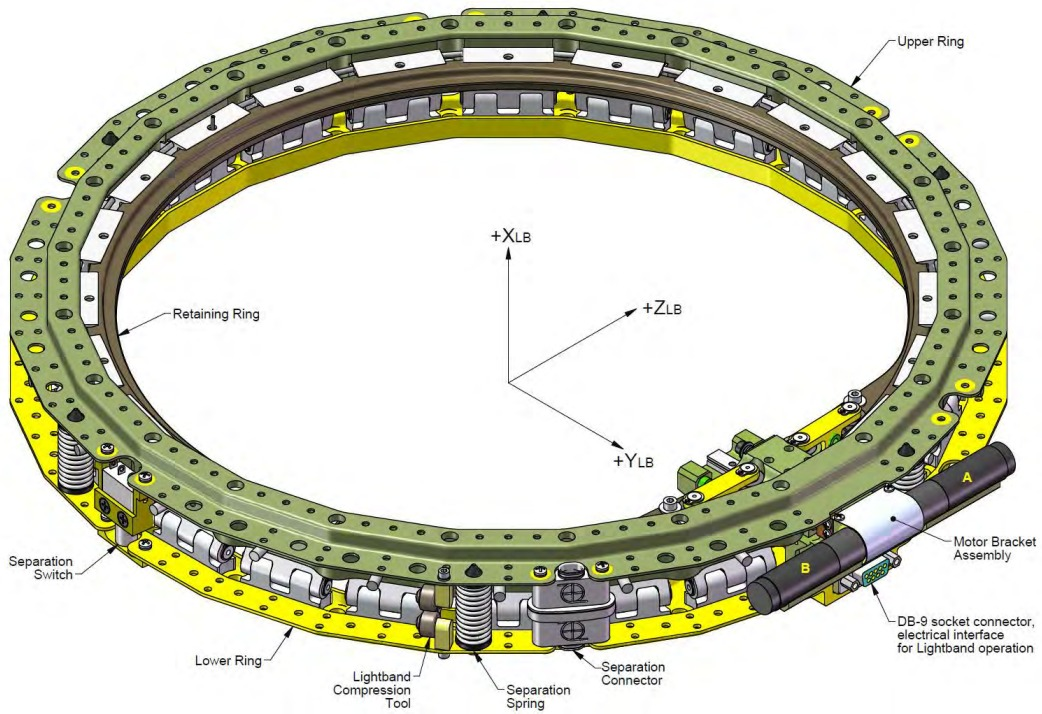
\includegraphics[width=0.65\linewidth]{PUCP_pictures/Motorized Lightband MkII.jpeg}
    \caption{Motorized Lightband MkII.}
    \label{fig:motorized_lightband_mkii}
\end{figure}

\begin{figure}[htbp]
    \centering
    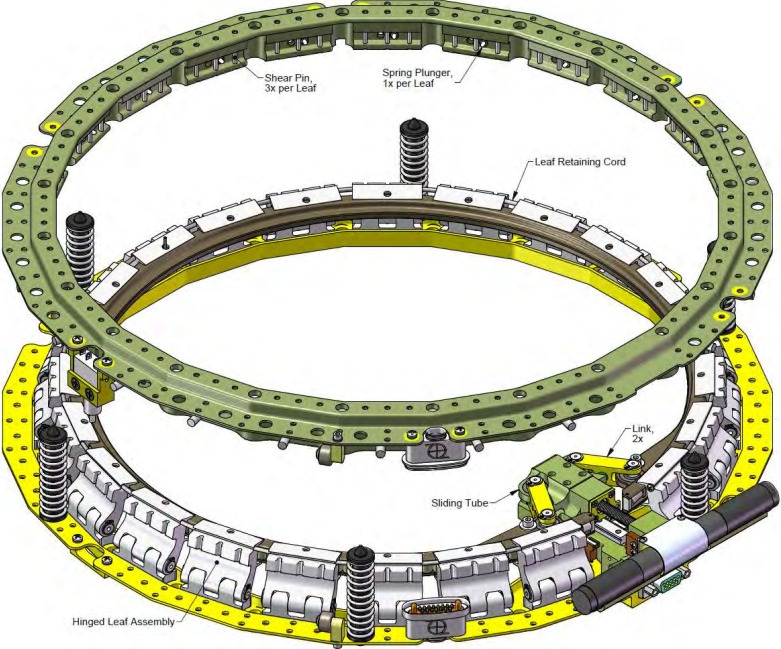
\includegraphics[width=0.65\linewidth]{PUCP_pictures/Moment of separation of the Motorized Lightband MkII.jpeg}
    \caption{Moment of separation of the Motorized Lightband MkII.}
    \label{fig:mlb_mkii_separation_moment}
\end{figure}

\begin{figure}[htbp]
    \centering
    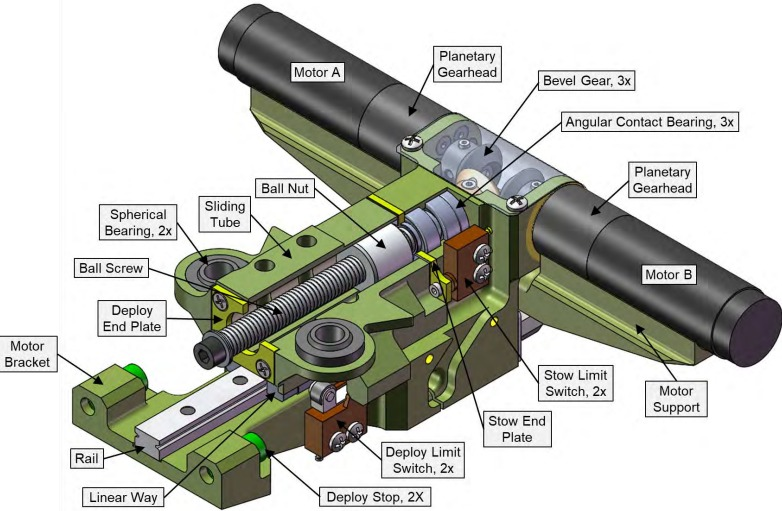
\includegraphics[width=0.65\linewidth]{PUCP_pictures/Gear–ball screw mechanism of the Motorized Lightband MkII.jpeg}
    \caption{Gear--ball screw mechanism of the Motorized Lightband MkII.}
    \label{fig:mlb_mkii_gear_ball_screw}
\end{figure}

\clearpage
\section{STARS-C Separation Mechanism}
\label{appsec:starsc_separation_mechanism}

The separation mechanism of the STARS-C project was based on springs and a resistive wire-cutting system \cite{Yamagiwa2017SpaceElevator}. The satellites were initially held together by Dyneema cables, which were severed upon receiving a command from Earth. The cutting process was achieved using a nichrome wire that, when electrically heated, melted the restraining cord and released the satellites.

After release, springs embedded within the CubeSat structure generated a separation force of approximately \(25~\mathrm{N}\), allowing the mother satellite and daughter satellite to move apart while deploying the tether from a spool located in the mother satellite. The system also incorporated a \(15~\mathrm{m}\) motorized reel to control the unwinding speed and reduce the risk of rebound or collision between both bodies at the end of the deployment process.

STARS-C was launched on December 9, 2016, from the International Space Station using the Japanese Kibo module. The mission represented an early in-orbit demonstration of tether deployment technology for small satellites.

\begin{figure}[htbp]
    \centering
    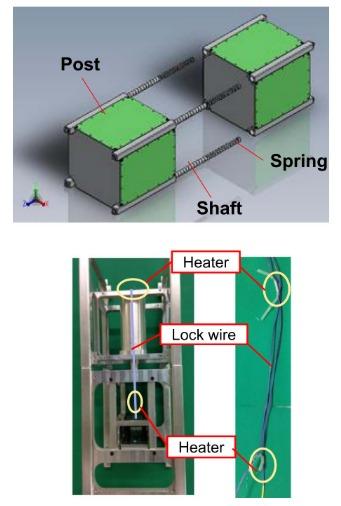
\includegraphics[width=0.4\linewidth]{PUCP_pictures/Separation mechanism of STARS-C.jpeg}
    \caption{Separation mechanism of STARS-C.}
    \label{fig:starsc_separation_mechanism}
\end{figure}

\begin{figure}[htbp]
    \centering
    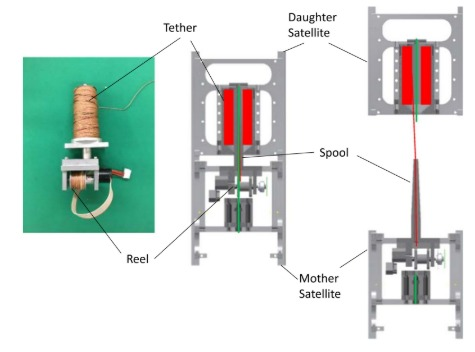
\includegraphics[width=0.5\linewidth]{PUCP_pictures/String release mechanism of STARS-C.jpeg}
    \caption{String release mechanism of STARS-C.}
    \label{fig:starsc_string_release_mechanism}
\end{figure}

\clearpage
\section{Explosive Bolt Separation Mechanism}
\label{appsec:explosive_bolt_separation}

Explosive bolts are mechanical fastening elements used to keep two structures joined until a trigger signal is applied \cite{Cui2015SatelliteSeparation}. Upon activation, a small pyrotechnic charge fractures the bolt cross-section, resulting in the immediate release of the joint. These mechanisms are commonly used in clamp-band separation systems, where the explosive bolt acts as the primary fastening element that keeps the assembly closed until deployment.

When the activation signal is received, the pyrotechnic charge inside the bolt is detonated, causing the bolt to rupture and allowing the retention ring to open. This releases the payload structure. Auxiliary springs are typically incorporated to ensure a uniform and complete separation between both parts of the joint. These springs provide the force required to prevent partially constrained regions that could compromise the separation process.

\begin{figure}[htbp]
    \centering
    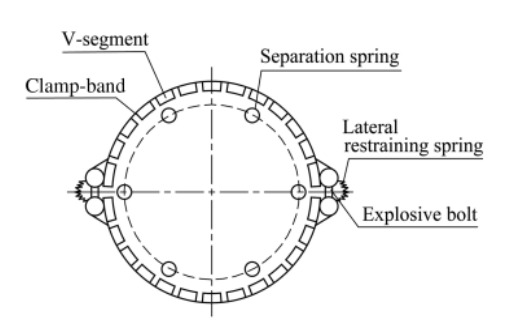
\includegraphics[width=0.5\linewidth]{PUCP_pictures/Clamp joining system.jpeg}
    \caption{Clamp joining system.}
    \label{fig:explosive_bolt_clamp_joining_system}
\end{figure}

\begin{figure}[htbp]
    \centering
    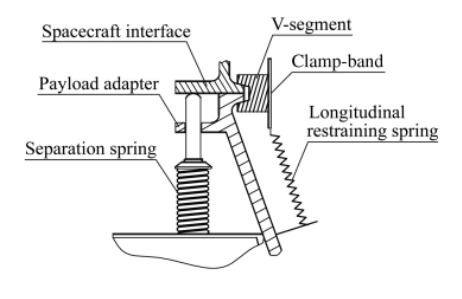
\includegraphics[width=0.5\linewidth]{PUCP_pictures/Locking system.jpeg}
    \caption{Locking system for clamp-band separation.}
    \label{fig:explosive_bolt_locking_system}
\end{figure}

\begin{figure}[htbp]
    \centering
    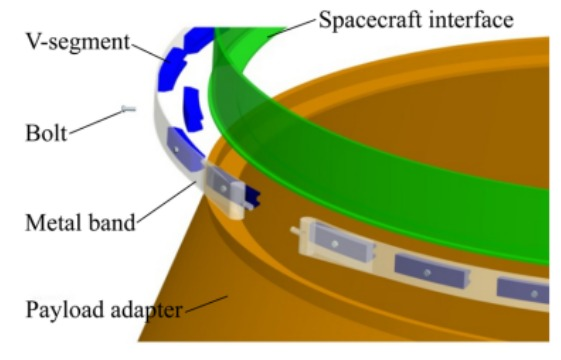
\includegraphics[width=0.5\linewidth]{PUCP_pictures/Clamp separation.jpeg}
    \caption{Clamp separation process.}
    \label{fig:explosive_bolt_clamp_separation}
\end{figure}

\clearpage
\section{CarboNIX NEO}
\label{appsec:carbonix_neo}

The CarboNIX NEO is a separation system developed by Exolaunch for small satellites of up to \(500~\mathrm{kg}\) \cite{Exolaunch2024CarboNIX}. It is a fully mechanical deployment mechanism based on retention rings and springs that store mechanical energy to provide the initial impulse to the payload during release.

The locking system of the CarboNIX NEO employs a redundant magnetic retention mechanism, complemented by an interlocking pin within the retention ring. This configuration provides the physical connection between the base and the payload until separation. During launch, permanent magnetic locks keep the ring closed without requiring continuous electrical power, while the interlocking pin acts as a mechanical safety feature to prevent unintended release.

Once the separation signal is issued, the magnetic locks are deactivated and the pin is retracted. This allows the retention ring to move due to the release of the springs. The motion activates a scissor-type mechanism that generates the final thrust required to release the payload.

\begin{figure}[htbp]
    \centering
    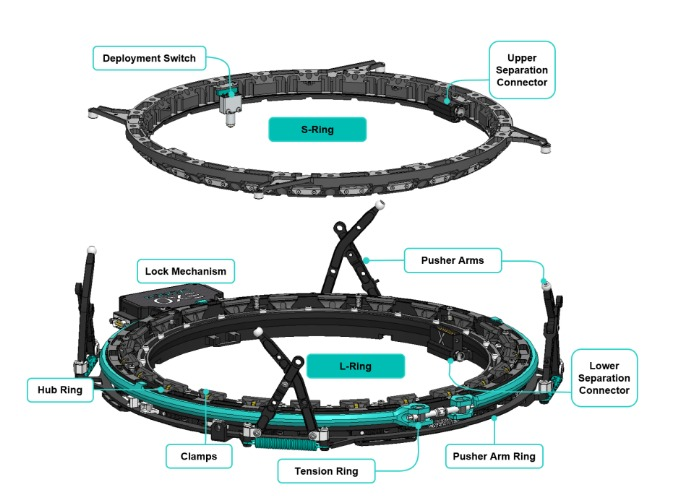
\includegraphics[width=0.6\linewidth]{PUCP_pictures/Separation moment of the CarboNIX.jpeg}
    \caption{Separation moment of the CarboNIX NEO.}
    \label{fig:carbonix_neo_separation_moment}
\end{figure}

\section{Comparison of Technologies}
\label{appsec:comparison_of_separation_technologies}

The separation systems analyzed in this appendix employ different methods for payload release and restraint. Table~\ref{tab:separation_technologies_comparison} summarizes the main characteristics of the reviewed technologies and their relevance to the LINKU separation mechanism.

\begin{table}[H]
\centering
\caption{Comparison of separation technologies for aerospace separation systems.}
\label{tab:separation_technologies_comparison}
\small
\renewcommand{\arraystretch}{1.3}

\begin{tabularx}{\textwidth}{|>{\centering\arraybackslash}X|
                              >{\centering\arraybackslash}X|
                              >{\centering\arraybackslash}X|
                              >{\centering\arraybackslash}X|
                              >{\centering\arraybackslash}X|}
\hline

\textbf{Aspect} & \textbf{Motorized Lightband MkII} & \textbf{STARS-C} & \textbf{Explosive Bolts} & \textbf{CarboNIX NEO} \\ \hline

Separation method & Electromechanical & Thermal release & Pyrotechnic release & Magnetic/mechanical release \\ \hline

Locking or restraint mechanism & Retention ring & Dyneema cord & Explosive bolt and clamp band & Magnetic retention and interlocking pin \\ \hline

Mechanical energy source & Preload springs & Springs & Auxiliary springs & Springs and scissor-type mechanism \\ \hline

Typical application & Commercial payload separation & Experimental tethered small satellite & Launch vehicle/payload separation & Commercial small-satellite deployment \\ \hline

Flight heritage & High flight heritage & Demonstrated in orbit & Commonly used in aerospace applications & High flight heritage for small-satellite deployment \\ \hline

Relevance to LINKU & Reliable but complex for LINKU scale & Relevant due to spring and thermal release concept & Effective but less suitable due to pyrotechnic complexity & Reliable but complex for LINKU scale \\ \hline

\end{tabularx}

\end{table}

\end{comment}



